\section{\protect\uppercase{Implementation}}

\subsection{Computational framework}

Peridigm is used in the context of the present study \cite{PeridigmUserGuide100}. It is an open-source computational state-based PD code developed at Sandia National Laboratories for massively-parallel multi-physics simulations. Peridigm uses a FE mesh as basis for its discretizations. Hexahedron and tetrahedron elements are transformed into peridynamic collocation points and associated with the respective element volume. Different material properties can be assigned by dividing the model into multiple blocks.

\subsection{Stochastic model}

To reduce possible dependencies of the solution from the underlying discretization scheme, a stochastic distribution of elastic material properties is proposed to incorporate the statistical nature of damage initiation (\autoref{fig:Thry:Stochastic:Implementation}). Additionally, this gives a possibility to check whether a failure pattern is driven by the chosen discretization or an actual phenomenon. \cite{SillingSA2007b} published a similar idea for capturing damage evolution by introducing fluctuations in the critical stretch by means of a Weibull or other distribution. The stochastic distribution of the elastic constants is also motivated by scatter in stress-strain curves and locations of failure of different test specimen and findings in micrographs in the bulk resin specimen (\autoref{fig:Exp:Tension}). These deviations may be caused by micro-voids, locally varying degree of cure in the epoxy material or slight disparities of the specimen geometries caused by the machining process. Introduction of a stochastic material distribution has the goal to filter and numerical effects in the simulation and to ensure, that the dominating effect causing the physical failure is adequately described in the numerical model. The calculations have to be performed multiple times with different stochastic distributions to assure the dominating effect is adequately triggered.

\begin{figure}[htbp]
  \setlength{\figheight}{5cm}
  \begin{subfigure}{0.49\linewidth}
    \begin{minipage}[b][\figheight]{\linewidth}
      \centering
      % Variables
      \def\nb{20}
      \def\ne{10}
      % Picture
      \begin{tikzpicture}
  \begin{axis}[
    width=\linewidth,
    height=\figheight,
    ybar,
    bar shift=0pt,
    %axis lines=middle,
    axis x line=bottom,
    axis y line=middle,
    samples=10,
    enlarge y limits=upper,
    xmin=-\ne/2-0.75,
    xmax= \ne/2+0.75,
    ymin=0,
    ymax=(\nb+1)*1.05,
    xlabel=$K$,
    ylabel=$n_e$,
    x label style={at={(axis description cs:1.0,0.0)},anchor=south west},
    y label style={at={(axis description cs:0.5,1.0)},anchor=south west},
    %xtick={-\ne/2,0,\ne/2},
    xtick={-5,0,5},
    ymajorticks=false,
    xticklabels={$\bar{K}-\Delta$,$\bar{K}$,$\bar{K}+\Delta$},
    yticklabels={},
  ]
    %\addplot +[black,fill=gray]{rnd};
    %\addplot coordinates {(-\ne/2,\nb)};
    \foreach \x in {-5,-4,...,5} {
      \addplot+[black,fill=gray] coordinates {(\x,\nb+rand)};%,bar shift=0.5
    }
  \end{axis}
\end{tikzpicture}
    \end{minipage}
    \caption{Simple stochastic model}
    \label{fig:Thry:Stochastic:Distribution}
  \end{subfigure}
  \hfill
  \begin{subfigure}{0.49\linewidth}
    \begin{minipage}[b][\figheight]{\linewidth}
      %\includegraphics[width=\linewidth,height=\figheight,keepaspectratio]{../../Material/Figures/Model_FE_Hex_0-5_Stochastic_ct.png}
      \includegraphics[width=\linewidth,height=\figheight,keepaspectratio]{Model_FE_Hex_0-5_Stochastic_ct}
    \end{minipage}
    \caption{Base FE mesh with stochastic block distribution}
    \label{fig:Thry:Stochastic:FEModel}
  \end{subfigure}
  \caption{Implementation of stochastic material distribution for PD simulations}
  \label{fig:Thry:Stochastic:Implementation}
\end{figure}

When Peridigm computes the internal force, it computes a force state at each node in the model and applies that force state to each bond that is attached to the node. For each bond, the resulting force density is applied to the node itself, and negative one times the force density is applied to the node on the other end of the bond.  This is consistent with the state-based formulation in \autoref{eq:PeridynamicLimits}. The way Peridigm handles material interfaces is basically a direct application of \autoref{eq:PeridynamicLimits}. The result at a material interface is an average of the two material models. Thus, a block-based stochastic model is possible by simply assigning materials with different elastic constants.

As the nature of the distribution of stochastic effects in the real specimen is currently unknown, a rather simple approach is chosen for their modeling. During the creation of the specimen, elements in the damage-prone area are stochastically associated to multiple block definitions. Each block is associated with a material that has a defined deviation from the nominal elastic constants. The number of different block definitions and the maximum deviation from the nominal elastic constants can be chosen randomly. More complex distribution, such as Gaussian or Weibull distribution, may be implemented in the future if the approach seems promising.

% % Weibull
% \begin{tikzpicture}
%   \def\a{10}
%   \def\b{1}
%   \begin{axis}[
%     smooth
%   ]
%     \addplot[domain=0:2,samples=100] {(\a/\b)*(x/\b)^(\a-1)*e^(-(x/\b)^\a)};
%   \end{axis}
% \end{tikzpicture}


% \href{http://imechanica.org/files/Silling_Peridynamic_McMat07.pdf}{http://imechanica.org/files/Silling\_Peridynamic\_McMat07.pdf}, Slide 20:
% 
% \cite{SillingSA2007b}
% 
% \begin{itemize}
%   \item We can introduce fluctuations in critical stretch as a function of position and bond orientation according to Weibull or other distribution.
%   \item This is one way of incorporating the statistical nature of damage evolution.
% \end{itemize}

